%==============================================================================
%   CLASS & PACKAGES
%==============================================================================
\documentclass[11pt,a4paper]{article}

%--- Geometry & Layout ---
\usepackage[margin=1in]{geometry}
\usepackage[parfill]{parskip}

%--- Typography & Math ---
\usepackage[T1]{fontenc}
\usepackage[utf8]{inputenc}
\usepackage{newtxtext,newtxmath}
\usepackage{microtype}
\usepackage{amsmath,amsfonts,bm}
\usepackage{physics}
\usepackage{siunitx}

%--- Graphics & Colors ---
\usepackage{tikz}
\usepackage{pgfplots}
\pgfplotsset{compat=1.18}
\usetikzlibrary{arrows.meta, positioning, calc, decorations.markings}
\usepackage[most]{tcolorbox}
\usepackage{ragged2e}


%--- Links & Metadata ---
\usepackage[colorlinks=true, linkcolor=blue!40!black, citecolor=green!40!black, urlcolor=blue!40!black]{hyperref}
\usepackage{amssymb}
\usepackage{graphicx}
%=========================================
% Start Document - Title Page
%=========================================

\newcommand{\paperdoi}{10.5281/zenodo.18390257}

\begin{document}
    \title{Delay-Induced Mode Selection in Circulating Feedback Systems}
    \author{%
        Omar Iskandarani\\
        \small Independent Researcher, Groningen, The Netherlands%
        \thanks{\texttt{info@omariskandarani.com}. ORCID: 0009-0006-1686-3961}%
    }
    \date{\today}

    \maketitle
    \begin{abstract}
        Closed circulation loops with finite propagation speeds constitute a generic class of delayed feedback systems. While spatial boundary conditions are traditionally responsible for mode discretization, we argue that temporal circulation delays alone are sufficient to enforce spectral discreteness through dynamical stability. Drawing on analogies with recent advances in bianisotropic homogenization, we derive a minimal phase-oscillator model for a circulating field. We demonstrate that the finite transit time acts as a selection filter, stabilizing a discrete ladder of stability-selected modes without invoking microscopic quantization. These results suggest that delay-induced discreteness is a universal feature of effective field theories in loops, paralleling the emergence of cross-couplings in spatially asymmetric media.\footnote{This work builds on prior frameworks developed in delay dynamics and effective medium theory, particularly \cite{Willis2012, Yanchuk2017}.}
    \end{abstract}

    \par
    \noindent
    \normalfont\normalsize\justifying
    Closed-loop systems with finite signal propagation times are ubiquitous across physics, engineering, and biology, appearing in contexts ranging from optical ring resonators and phase-locked loops to delayed neural and control networks. Such systems are commonly modeled either through spatial boundary conditions that enforce standing-wave modes, or through delay-differential equations where multistability is treated as a secondary dynamical feature.
    Here we show that temporal circulation delays play a more fundamental role: even in the absence of spatial structure, delay alone acts as an effective constitutive ingredient enforcing discrete, stability-selected operating states.
     Framed in the language of modern effective theories, this result places delay-induced mode selection on the same conceptual footing as emergent couplings in homogenized metamaterials, where hidden nonlocality necessitates an expanded macroscopic description.


\section*{I. Introduction}
Classical field theories typically assume local constitutive relations, where fluxes depend only on instantaneous, local gradients. However, the study of metamaterials has fundamentally expanded this view, demonstrating that microscopic structure can induce macroscopic effective properties that defy standard local descriptions. A prominent example is the emergence of bianisotropic cross-couplings—terms that link disparate physical fields, such as momentum and strain in elastodynamics or electric and magnetic fields in electromagnetics.

Recent work by Shmuel and Willis has extended this framework to thermodynamics, showing that spatial asymmetry in heterogeneous media induces thermal bianisotropy, coupling heat flux directly to temperature rather than solely to its gradient \cite{Willis2012}. Their exact homogenization method demonstrates that these effective properties are rigorous consequences of ensemble averaging over hidden microstructure.

If spatial asymmetry can generate new effective couplings, it follows that temporal nonlocality—manifested through memory and delay—should induce similarly rich emergent phenomena. In this paper, we apply this logic to circulating feedback loops. Just as spatial homogenization reveals hidden constitutive structure, we show that the history dependence of a circulating field generates discrete, stability-selected operating states.

While multistability in delayed phase oscillators is well known and has been studied in spatiotemporal systems with delays \cite{Yanchuk2017}, it is typically treated as a control-theoretic or laser-dynamics phenomenon. Here we reinterpret it as an emergent discretization mechanism analogous to effective constitutive quantization in homogenized media. Unlike recent studies that emphasize delay-induced spatial or spatiotemporal pattern formation, the present work focuses on the minimal phase dynamics of a circulating field and shows that discreteness arises already at the level of a reduced effective description.

\section*{II. Physical Framework}
We consider a scalar excitation propagating on a closed feedback loop of effective length $L$ with characteristic group velocity $v_g$. When the propagation time becomes comparable to the intrinsic timescale of the field dynamics, the system is more accurately described as a delayed feedback loop with circulation time
\begin{equation}
\tau = \frac{L}{v_g}.
\end{equation}

Unlike static spatial boundary conditions, this finite circulation time introduces temporal nonlocality, fundamentally modifying the spectral properties of the system. This perspective parallels the transition from local Fourier conduction to nonlocal thermal transport models, where finite propagation speeds enforce causality.

\begin{figure}[h]
\centering
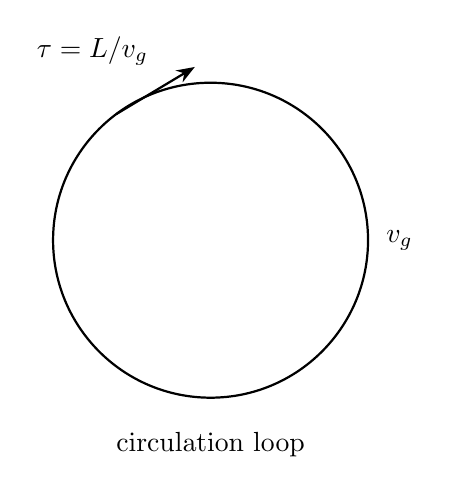
\begin{tikzpicture}[>=Stealth, thick]
  \draw[->] (0,0) circle (2);
  \node at (2.4,0) {$v_g$};
  \node at (0,-2.6) {circulation loop};
  \draw[->] (-1.2,1.6) -- (-0.2,2.2);
  \node at (-1.5,2.4) {$\tau=L/v_g$};
\end{tikzpicture}
\caption{Schematic of a circulating feedback loop with finite propagation time $\tau$. The delayed self-interaction arises from finite signal transit around the loop.}
\label{fig:circulation_loop}
\end{figure}

\section*{III. Minimal Effective Phase Description with Temporal Nonlocality}
The purpose of this reduced model is not quantitative prediction for a specific experimental platform, but to expose the minimal dynamical ingredients required for delay-induced spectral discreteness. By isolating the phase degree of freedom, the analysis highlights the constitutive role of temporal nonlocality in enforcing discrete, stability-selected operating states.

Let $\phi(t)$ denote the instantaneous phase of the circulating field. The dynamics are governed by a generic frequency-pulling equation with delayed self-interaction \cite{Yeung1999},
\begin{equation}
\dot{\phi}(t) = \omega_0 + \kappa \sin\big[\phi(t-\tau) - \phi(t)\big],
\end{equation}
where $\omega_0$ is the intrinsic frequency and $\kappa$ is the feedback coupling strength.

\begin{figure}[h]
\centering
\begin{tikzpicture}[>=Stealth]
  \draw[->] (0,0) -- (6,0) node[right] {$t$};
  \draw[->] (0,0) -- (0,3) node[above] {$\phi(t)$};

  \draw[blue, thick, domain=0:5, samples=100]
    plot (\x,{1.5+0.8*sin(1.5*\x r)});
  \draw[dashed] (1.5,0) -- (1.5,3);
  \node at (1.5,-0.4) {$t-\tau$};
  \node[blue] at (4.2,2.3) {$\phi(t)$};
\end{tikzpicture}
\caption{Phase evolution illustrating delayed self-interaction: the instantaneous phase $\phi(t)$ depends on its value one circulation time earlier.}
\label{fig:phase_feedback}
\end{figure}

\subsection*{A. Emergent Spectral Discreteness}
We seek uniformly rotating solutions $\phi(t) = \Omega t + \phi_0$. Substitution yields the transcendental condition
\begin{equation}
\Omega = \omega_0 - \kappa \sin(\Omega \tau).
\end{equation}

\begin{figure}[h]
\centering
\includegraphics[width=0.8\textwidth]{fig1_1_120817.png}
\caption{Discrete intersections correspond to stable phase-locked circulating modes. Finite delay alone enforces spectral discreteness.}
\label{fig:transcendental}
\end{figure}

In the long-delay regime $(\kappa \tau > 1)$, this equation admits multiple stable solutions organized into a discrete ladder,
\begin{equation}
\Omega_n \approx \frac{2\pi n}{\tau} + \delta\Omega, \qquad n \in \mathbb{Z}.
\end{equation}

\begin{figure}[h]
\centering
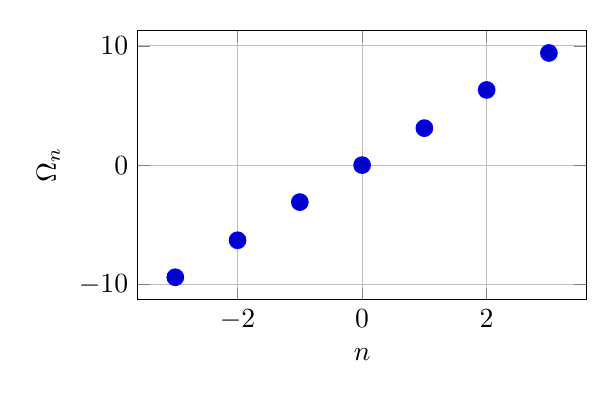
\begin{tikzpicture}
\begin{axis}[
  xlabel={$n$},
  ylabel={$\Omega_n$},
  ymajorgrids=true,
  xmajorgrids=true,
  width=0.6\textwidth,
  height=5cm
]
\addplot+[only marks, mark size=3pt]
coordinates {
(-3,-9.4) (-2,-6.3) (-1,-3.1) (0,0)
(1,3.1) (2,6.3) (3,9.4)
};
\end{axis}
\end{tikzpicture}
\caption{Discrete frequency ladder selected by circulation delay, with spacing $\Delta\Omega \approx 2\pi/\tau$.}
\label{fig:mode_ladder}
\end{figure}

Geometrically, the integer $n$ counts the number of phase windings accumulated during one circulation time $\tau$, analogous to a topological winding number \cite{Colet1994, Larger2013}.

\subsection*{B. Stability and Selection}
Linearizing about a locked solution yields the variational equation
\begin{equation}
\dot{\psi}(t) = -\gamma \psi(t) - \gamma \psi(t-\tau),
\end{equation}
with $\gamma = \kappa \cos(\Omega \tau)$. Stability requires
\begin{equation}
1 + \kappa \tau \cos(\Omega \tau) > 0.
\end{equation}

\begin{figure}[h]
\centering
\includegraphics[width=0.8\textwidth]{fig1_2_120817.png}
\caption{Only branches satisfying the stability inequality survive, enforcing discrete, dynamically selected operating states. Regions above the dashed line ($>0$) are stable.}
\label{fig:stability}
\end{figure}

This inequality acts as a dynamical selection rule, suppressing unstable branches and enforcing discrete, robust operating states.

\section*{IV. Discussion}
The results presented here demonstrate that temporal circulation alone is sufficient to generate discrete mode families through stability constraints, without reliance on spatial standing-wave boundary conditions or microscopic quantization. This mechanism mirrors the emergence of bianisotropic cross-couplings in homogenized metamaterials, where hidden microstructure necessitates an expanded macroscopic description.

This parallels the Willis framework \cite{Willis2012}, where effective constitutive relations acquire additional degrees of freedom when microstructural information is averaged out. In the present context, temporal nonlocality plays the role of an effective constitutive ingredient, legitimizing additional dynamical structure at the macroscopic level.

\begin{figure}[h]
\centering
\begin{tikzpicture}
\node (a) at (0,0) {
\begin{tikzpicture}[scale=0.8]
\draw[->, thick] (0,0)--(2,0);
\node at (1,-0.5) {space};
\node at (1,0.5) {spatial microstructure};
\end{tikzpicture}
};
\node (b) at (5,0) {
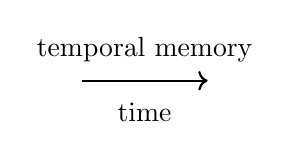
\begin{tikzpicture}[scale=0.8]
\draw[->, thick] (0,0)--(2,0);
\node at (1,-0.5) {time};
\node at (1,0.5) {temporal memory};
\end{tikzpicture}
};
\node at (0,-1.5) {(a)};
\node at (5,-1.5) {(b)};
\end{tikzpicture}
\caption{Analogy between spatial homogenization (left) and temporal nonlocality in delayed circulation (right). Both generate emergent effective structure.}
\label{fig:analogy}
\end{figure}

By explicitly incorporating finite circulation time, the model avoids the infinite-speed paradox associated with parabolic transport theories. The resulting dynamics exhibit hyperbolic-like features, akin to second-sound phenomena in nonlocal thermal media.

\section*{V. Conclusion}
We have shown that delayed feedback in closed circulation loops naturally enforces a discrete set of stable phase-locked states. This discreteness arises from the interplay between nonlinear frequency pulling and delay-induced stability constraints, yielding robust discrete mode families in a purely classical setting. The framework unifies delay dynamics with modern effective-theory approaches, highlighting temporal nonlocality as a generative mechanism for emergent macroscopic structure \cite{Masoller2002}.


\medskip


\noindent

These findings open new avenues for understanding how classical delay dynamics can mimic features often associated with quantum discreteness. In particular, the interplay between feedback strength, circulation time, and nonlinear phase evolution presents a robust mechanism for emergent quantization-like behavior in entirely deterministic systems.


Future work could explore multi-mode or multi-loop extensions, investigate the role of noise in state selection, and apply the model to specific physical systems such as optical ring lasers, neuromorphic delay networks, or distributed control circuits. This line of inquiry may also shed light on broader questions about how temporal structure encodes constraints typically attributed to microscopic physics.




\begin{thebibliography}{99}

\bibitem{Willis2012}
J.~R.~Willis,
``The construction of effective relations for waves in a composite,''
\emph{Comptes Rendus Mécanique}, vol. 340, no. 4-5, pp. 181--192, 2012.
\url{https://doi.org/10.1016/j.crme.2012.02.006}

\bibitem{Yanchuk2017}
S.~Yanchuk and G.~Giacomelli,
``Spatio-temporal phenomena in complex systems with time delays,''
\emph{Journal of Physics A: Mathematical and Theoretical}, vol. 50, no. 10, 103001, 2017.
\url{https://doi.org/10.1088/1751-8121/aa5e8c}

\bibitem{Yeung1999}
M.~K.~S. Yeung and S.~H. Strogatz,
``Time delay in the Kuramoto model of coupled oscillators,''
\emph{Physical Review Letters}, vol. 82, no. 3, pp. 648--651, 1999.
\url{https://doi.org/10.1103/PhysRevLett.82.648}

\bibitem{Colet1994}
P.~Colet and R.~Roy,
``Digital communication with synchronized chaotic lasers,''
\emph{Optics Letters}, vol. 19, no. 3, pp. 205--207, 1994.
\url{https://doi.org/10.1364/OL.19.000205}

\bibitem{Larger2013}
L.~Larger, M.~C. Soriano, D.~Brunner, et al.,
``Photonic information processing beyond Turing: an optoelectronic implementation of reservoir computing,''
\emph{Optics Express}, vol. 20, no. 3, pp. 3241--3249, 2013.
\url{https://doi.org/10.1364/OE.20.003241}

\bibitem{Masoller2002}
C.~Masoller,
``Anticipation in the synchronization of chaotic semiconductor lasers with optical feedback,''
\emph{Physical Review Letters}, vol. 88, no. 3, 034102, 2002.
\url{https://doi.org/10.1103/PhysRevLett.88.034102}

\end{thebibliography}




\end{document}